\documentclass{beamer}

\usepackage[utf8]{inputenx}
\usepackage{csquotes}
\usepackage{microtype}
\usepackage{graphicx}
\usepackage[absolute, overlay]{textpos}
\setlength{\TPHorizModule}{\paperwidth}
\setlength{\TPVertModule}{\paperheight}

\usetheme{UNC}

\author{Lianrui Geng \and Shengkai Tao}
\title{State Energy Lifestyle Profiles}
\subtitle{A Mini Design Study --- COMP 617}
\date{April 2025}


\begin{document}


%% Slide 1: Outline
\section{Overview}
\begin{frame}
    \frametitle{Outline}
    \tableofcontents
\end{frame}


%% Slide 2: Step 1 --- Learning
\section{Precondition}
\begin{frame}
    \frametitle{Step 1 --- Learning}

    \textbf{Question:}
    Do U.S.\ states exhibit different \alert{lifestyle profiles} through their energy consumption structures?

    \bigskip

    \begin{itemize}
        \item Total rankings hide \emph{how} energy is used day-to-day

        \medskip
        \item Sector breakdown (Residential, Commercial, Industrial, Transportation) reveals structural patterns that totals obscure

        \medskip
        \item \textbf{Stakeholder:} general public \& community advocates who want an intuitive way to compare states beyond aggregate numbers
    \end{itemize}
\end{frame}


%% Slide 3: Step 2 --- Winnowing
\begin{frame}
    \frametitle{Step 2 --- Winnowing}

    \begin{block}{Source}
        CORGIS / U.S.\ EIA SEDS \quad---\quad 51 states, 2010--2019
    \end{block}

    \medskip

    \textbf{Columns used (per sector):}
    \begin{itemize}
        \item Coal, Natural Gas, Petroleum, Wood, Geothermal, etc.
        \item Summed into 4 sector totals $\rightarrow$ normalized to \textbf{\% shares}
    \end{itemize}

    \medskip

    \textbf{Why necessary \& sufficient:}
    \begin{itemize}
        \item State + Year identify each unit; 4 sector shares define the profile
        \item Shares remove state-size effect, enabling fair comparison
    \end{itemize}

    \medskip

    \textbf{Bias:} \alert{Direct-fuel only} --- electric-heating states appear lower in Residential; missing values coded as 0
\end{frame}


%% Slide 4: Step 3 --- Discover
\section{Core}
\begin{frame}
    \frametitle{Step 3 --- Discover}

    \textbf{Process:} Stakeholder wants to compare states (horizontal) and check stability (longitudinal) $\rightarrow$ two core tasks; Task 3 added after iteration feedback

    \bigskip

    \begin{block}{Task 1 --- Cross-State Comparison}
        \textbf{Action:} Compare \quad \textbf{Target:} Distribution \\
        Compare sector share profiles across all states in a selected year
    \end{block}

    \medskip

    \begin{block}{Task 2 --- Temporal Trend}
        \textbf{Action:} Identify trends \quad \textbf{Target:} Change over time \\
        Track how one state's profile shifts over 2010--2019
    \end{block}

    \medskip

    \begin{block}{Task 3 --- Spatial Outliers \small{(from iteration)}}
        \textbf{Action:} Identify \quad \textbf{Target:} Outliers / spatial patterns \\
        Find extreme-share states and locate them geographically
    \end{block}
\end{frame}


%% Slide 5: Step 4 --- Design
\begin{frame}
    \frametitle{Step 4 --- Design}

    \begin{columns}[T]
        \begin{column}{0.50\textwidth}
            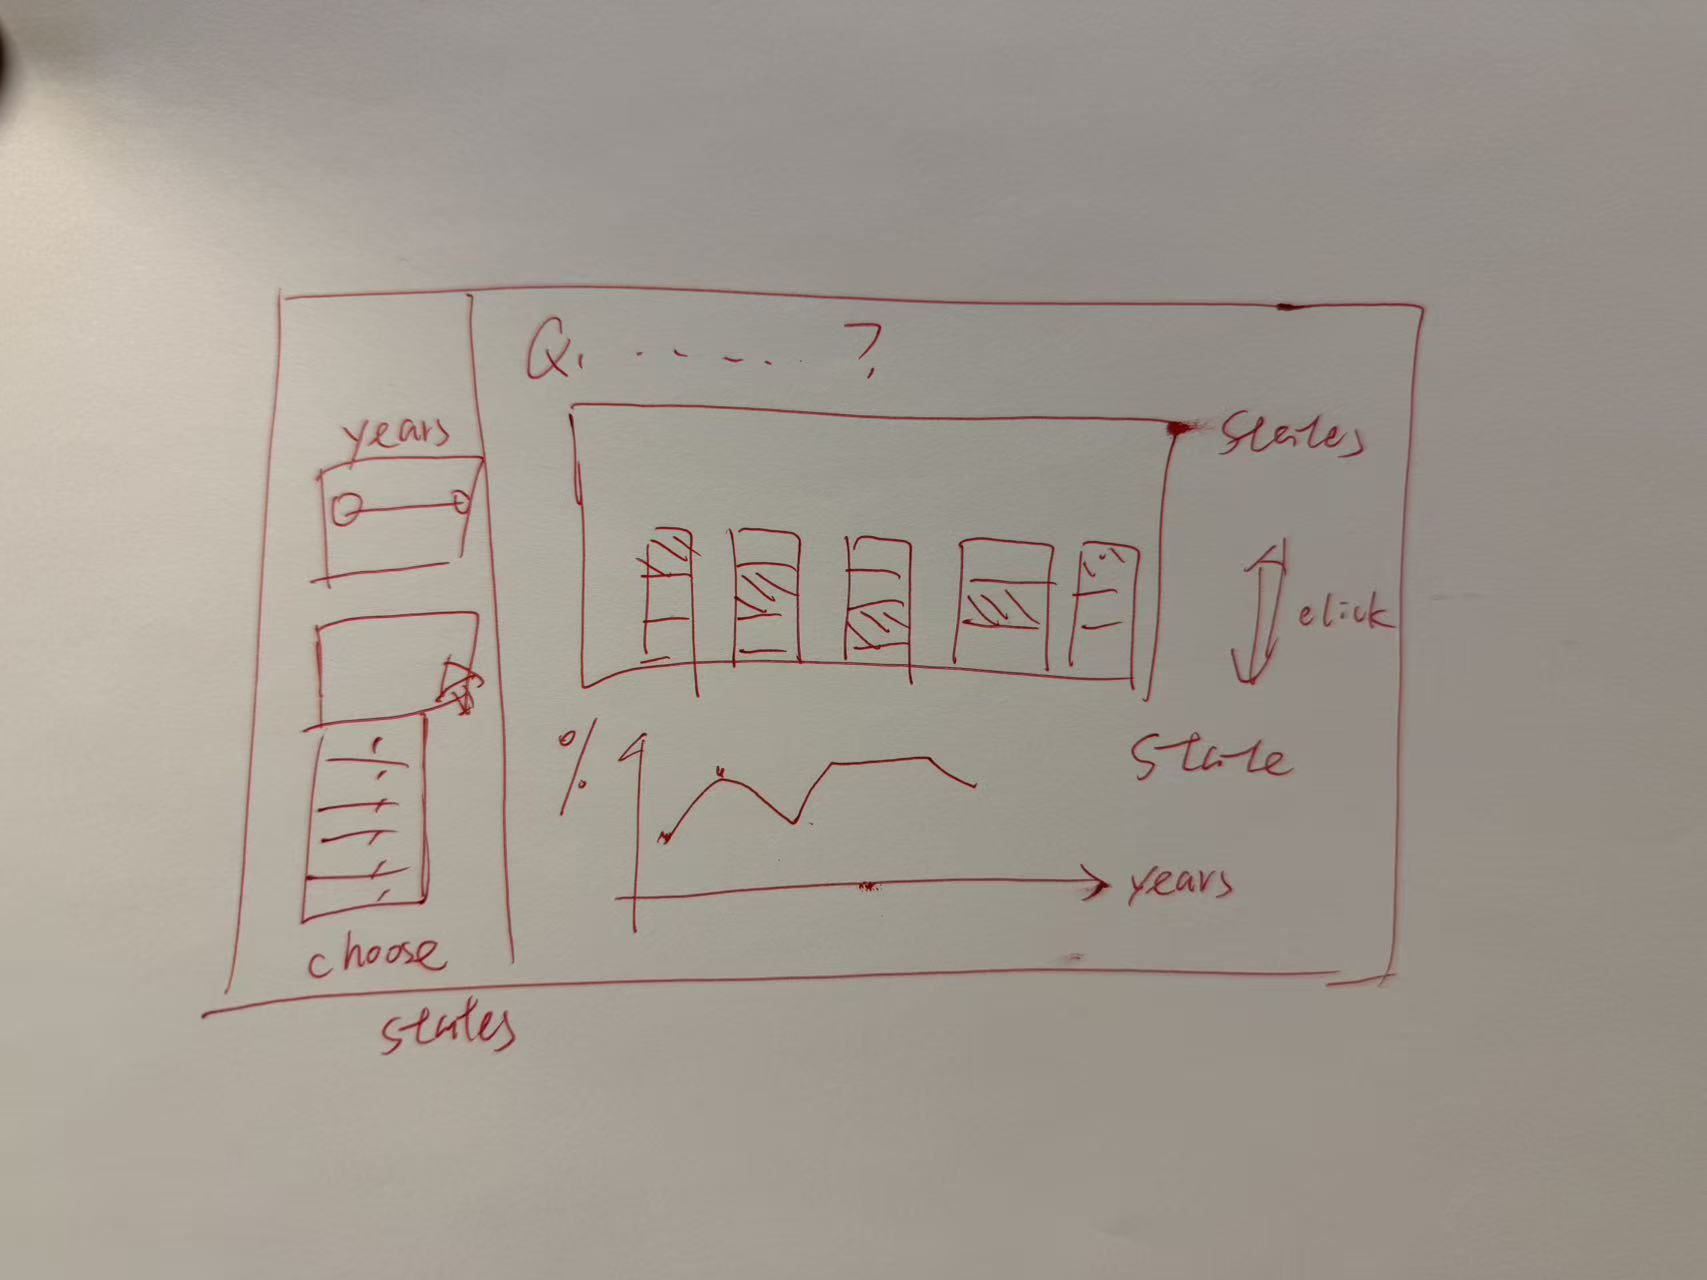
\includegraphics[width=\textwidth]{images/sketch.jpg}
        \end{column}
        \begin{column}{0.46\textwidth}
            \textbf{Justifications:}
            \begin{itemize}
                \item Stacked bar $\rightarrow$ supports Task 1 (compare distributions)
                \item Line chart $\rightarrow$ supports Task 2 (trends)
                \item Click bar to update detail $\rightarrow$ overview-to-detail workflow
                \item \% shares over raw totals $\rightarrow$ easier for public audience
            \end{itemize}

            \medskip

            \textbf{Trade-off:} middle segments hard to compare; sorting \& tooltips mitigate
        \end{column}
    \end{columns}
\end{frame}


%% Slide 6: Step 5 --- Implement (Map)
\begin{frame}
    \frametitle{Step 5 --- Implement: Map View}

    \begin{center}
        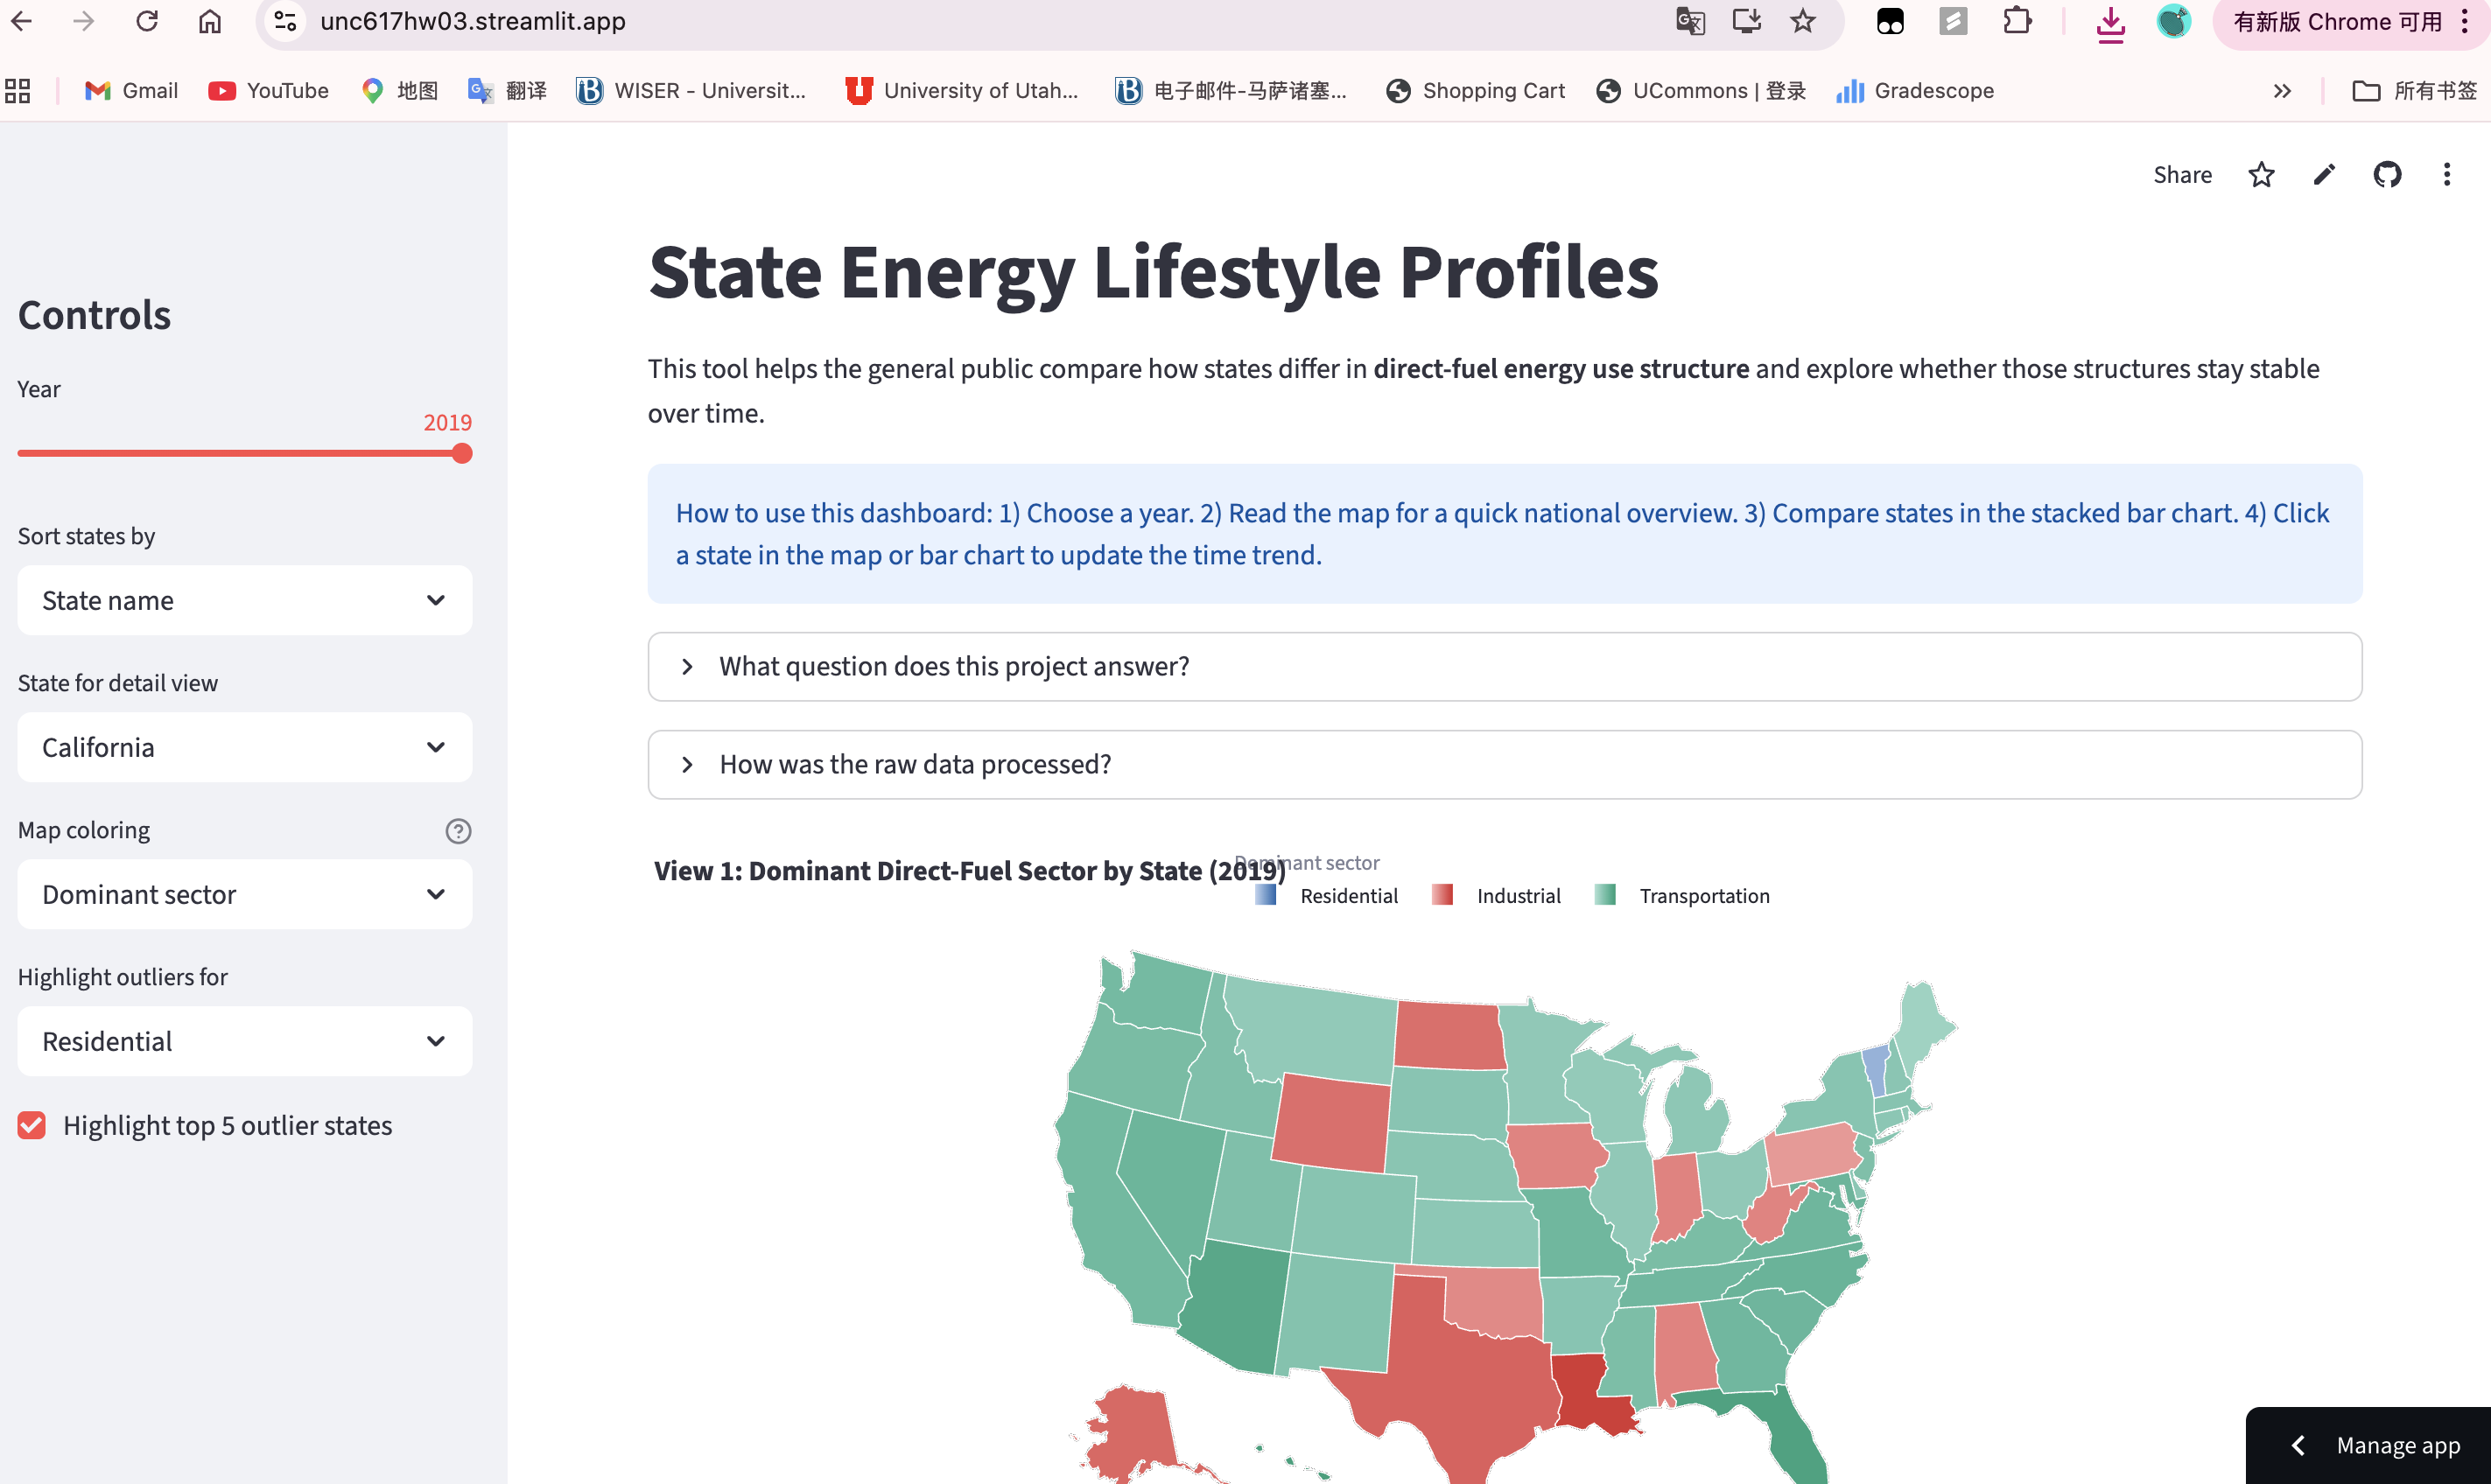
\includegraphics[width=0.95\textwidth]{images/dashboard01.png}
    \end{center}

    \smallskip
    \centering\small Streamlit + Plotly + Pandas \quad|\quad Choropleth addresses Task 3 (spatial outliers)
\end{frame}


%% Slide 7: Step 5 --- Implement (Bar & Line)
\begin{frame}
    \frametitle{Step 5 --- Implement: Bar \& Trend Views}

    \begin{columns}[T]
        \begin{column}{0.50\textwidth}
            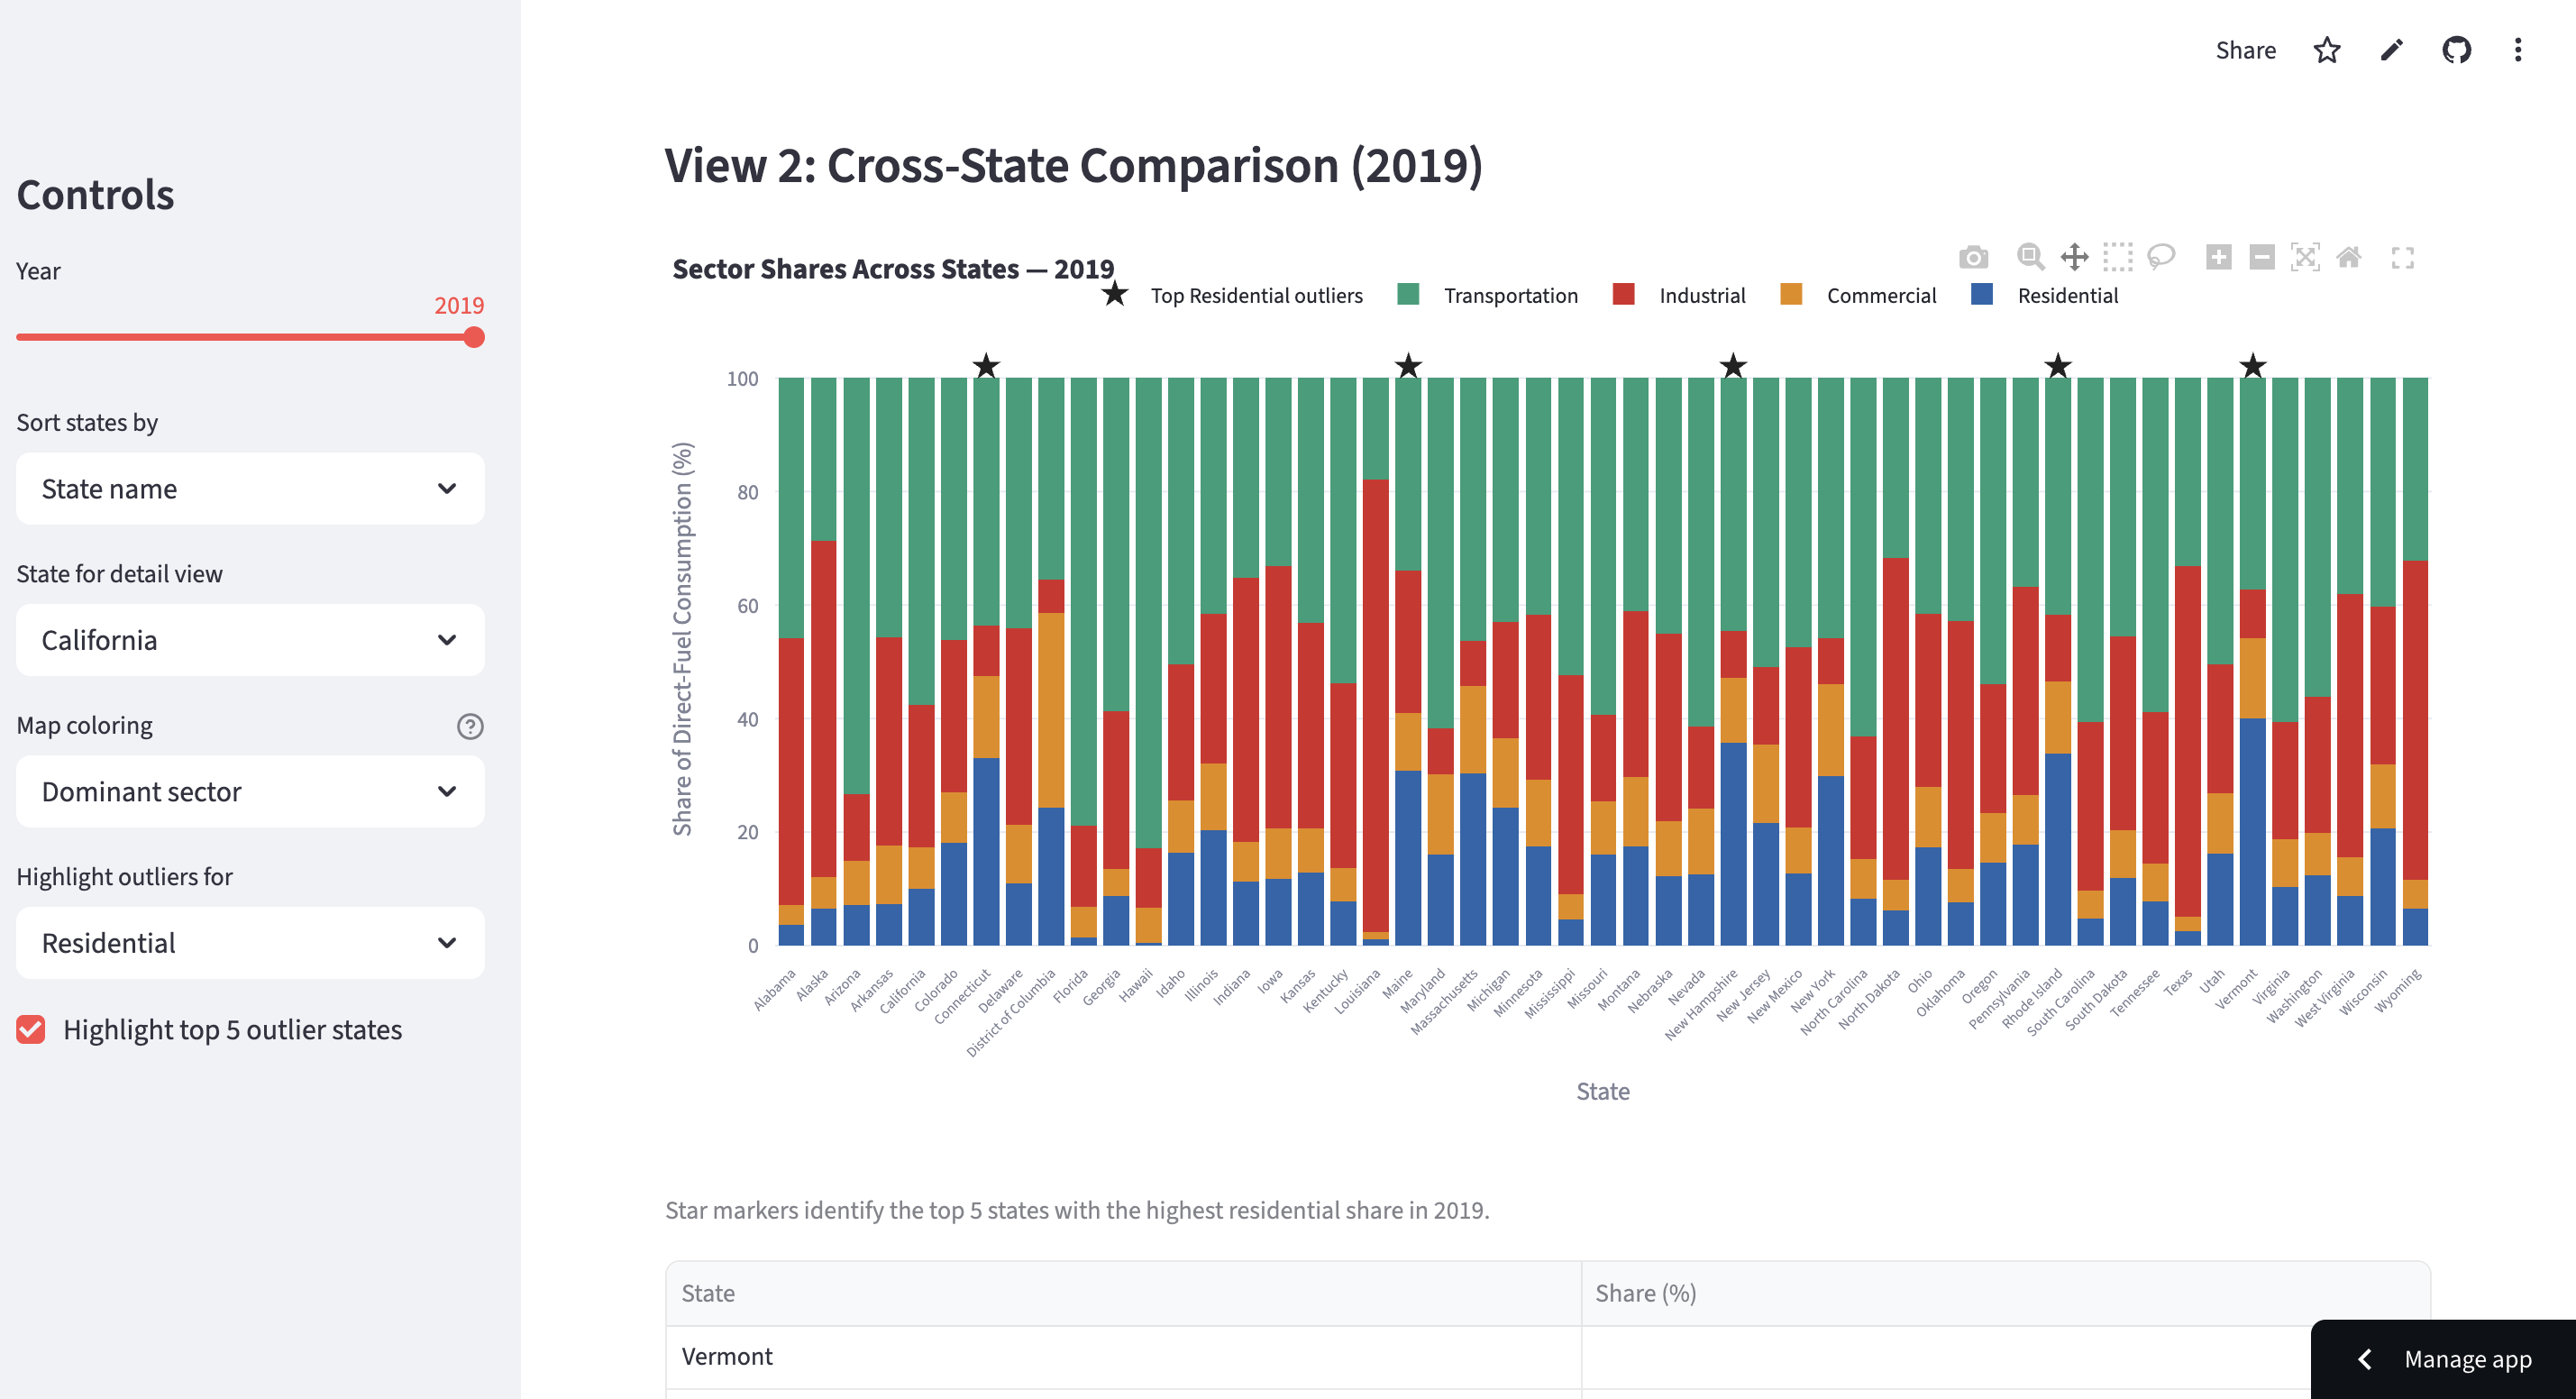
\includegraphics[width=\textwidth]{images/dashboard02.png}
            \centering\small Task 1: stacked bar + outlier stars
        \end{column}
        \begin{column}{0.50\textwidth}
            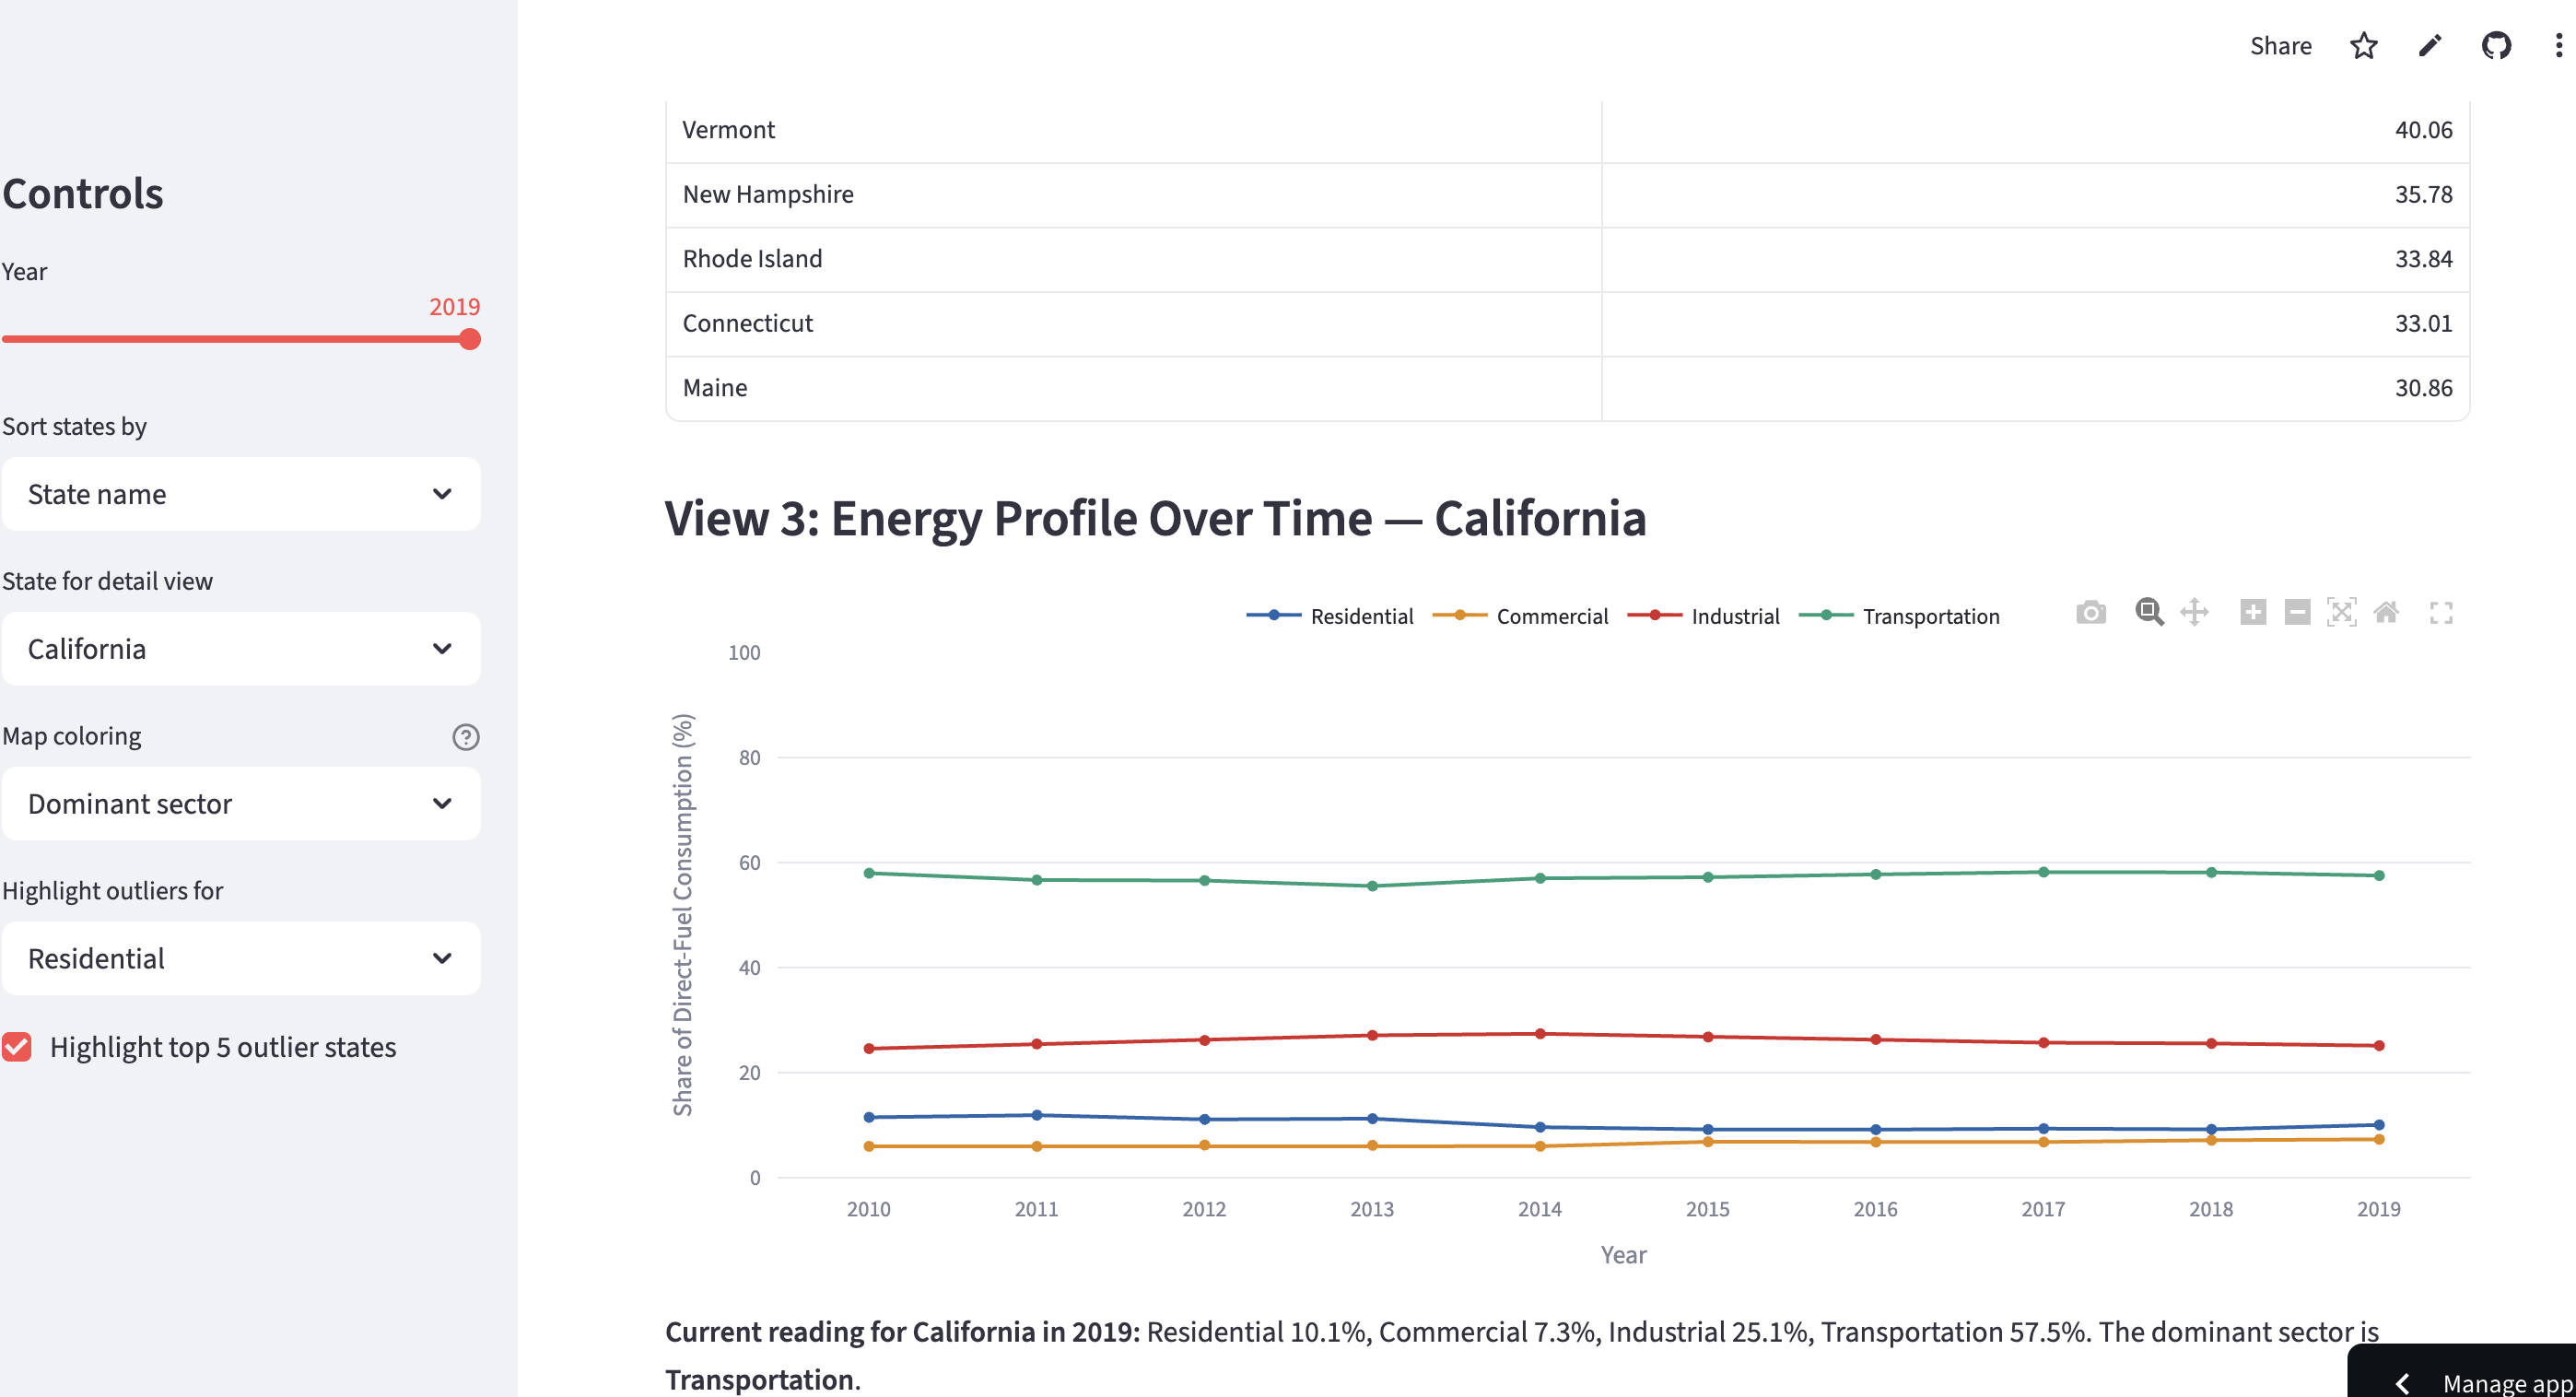
\includegraphics[width=\textwidth]{images/dashboard03.png}
            \centering\small Task 2: temporal trend (California)
        \end{column}
    \end{columns}

    \bigskip

    \centering\small Beyond defaults: custom palette, sortable axis, coordinated views, onboarding text
\end{frame}


%% Slide 8: Steps 6 & 7 --- Deploy & Iterate
\begin{frame}
    \frametitle{Steps 6 \& 7 --- Deploy \& Iterate}

    \textbf{Stakeholder observations during deployment:}
    \begin{itemize}
        \item Northeast (Maine, Vermont): higher Residential share --- direct-fuel heating
        \item Gulf states (TX, LA): stronger Industrial \& Transportation
        \item Most profiles stable over 2010--2019
    \end{itemize}

    \bigskip

    \textbf{Formative feedback (3/31):}
    \begin{itemize}
        \item Research question not obvious at first glance
        \item Need a \alert{U.S.\ map} for spatial context
    \end{itemize}

    \bigskip

    \textbf{Response:} Added choropleth map, onboarding text, outlier highlights $\rightarrow$ Task 3
\end{frame}


%% Slide 9: Step 8 --- Reflect Pt 1
\section{Analysis}
\begin{frame}
    \frametitle{Step 8 --- Reflect: Evaluation}

    \textbf{Method (4/7):} think-aloud exploration with classmate stakeholders

    \medskip

    \textbf{What the tool reveals:} States differ not just in \emph{how much} energy they use, but in \emph{how} they use it --- regional patterns emerge that totals alone cannot show

    \bigskip

    \begin{columns}[T]
        \begin{column}{0.46\textwidth}
            \textbf{Worked well}
            \begin{itemize}
                \item Map immediately intuitive
                \item Coordinated views: overview $\rightarrow$ detail
            \end{itemize}
        \end{column}
        \begin{column}{0.46\textwidth}
            \textbf{Could improve}
            \begin{itemize}
                \item Assumed too much prior knowledge
                \item Controls not obviously interactive
            \end{itemize}
        \end{column}
    \end{columns}

    \bigskip

    \textbf{Future:} annotation callouts, richer tooltips, climate/infrastructure overlays
\end{frame}


%% Slide 10: Step 9 --- Reflect Pt 2
\begin{frame}
    \frametitle{Step 9 --- Reflect: Design Lessons}

    \begin{enumerate}
        \item \textbf{Framing is part of the design} \\
              Charts fail if users don't know what question they answer

        \bigskip
        \bigskip

        \item \textbf{Coordinated views help unfamiliar domains} \\
              Map $\rightarrow$ bars $\rightarrow$ line guided different reasoning stages

        \bigskip
        \bigskip

        \item \textbf{Signpost all interactions} \\
              Users should never guess what is clickable

        \bigskip
        \bigskip

        \item \textbf{Stakeholder feedback reshapes design} \\
              Shifted from analytical to interpretable --- a major improvement
    \end{enumerate}
\end{frame}


%% Slide 11: Thanks
\begin{frame}
    \centering

    \vspace{2cm}

    {\LARGE \textbf{Thanks for Listening!}}

    \bigskip
    \bigskip

    Lianrui Geng \quad\&\quad Shengkai Tao

    \medskip

    \small COMP 617 --- April 2025
\end{frame}


\end{document}
